% ====================================================================
% oversamplingChain.tex
% --------------------------------------------------------------------
% Block diagram of oversampling and averaging, drawn with plain TikZ.
% ====================================================================

\begin{figure}[htbp]
\centering
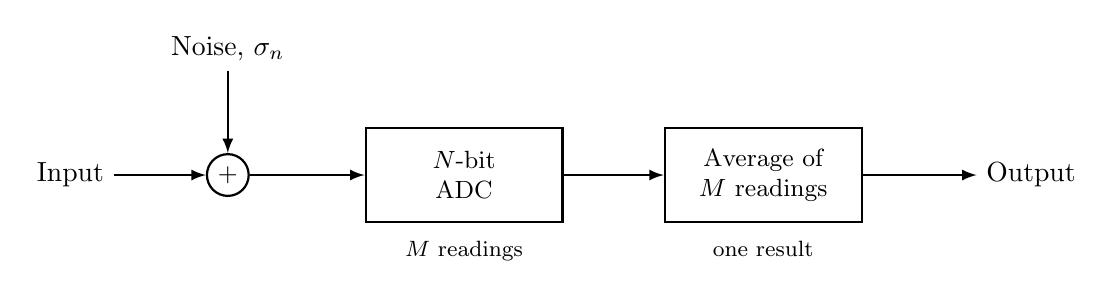
\begin{tikzpicture}[
  block/.style={draw, thick, minimum width=2.5cm, minimum height=1.2cm,
                align=center, font=\small},
  sum/.style={draw, thick, circle, inner sep=2pt, font=\small},
  >=latex
]
  \node (in) at (0,0) {Input};
  \node[sum]   (add) at (2.0,0)  {$+$};
  \node[block] (adc) at (5.0,0)  {$N$-bit\\ADC};
  \node[block] (avg) at (8.8,0)  {Average of\\$M$ readings};
  \node (out) at (12.2,0) {Output};
  \node (noise) at (2.0,1.6) {Noise, $\sigma_n$};

  \draw[->, thick] (in) -- (add);
  \draw[->, thick] (noise) -- (add);
  \draw[->, thick] (add) -- (adc);
  \draw[->, thick] (adc) -- (avg);
  \draw[->, thick] (avg) -- (out);

  \node[font=\footnotesize, below=3pt] at (adc.south) {$M$ readings};
  \node[font=\footnotesize, below=3pt] at (avg.south) {one result};
\end{tikzpicture}
\caption{Oversampling and averaging. The converter takes $M$ readings for
each output sample, and the output is their mean.}
\label{fig:oversamplingChain}
\end{figure}
